\chapter{Design and Implementation}

\epigraph{\textit{... where in this snippet $W1$ and $W2$ are two matrices that we initialize randomly. We're not using biases because meh.}}{\rightline{{\rm --- Andrej Karpathy}}}

After researching literature on building libraries from scratch, analyzing pet project source-codes \cite{convnetjs, gibianskysource} and dozens of implementations of professional libraries \cite{TF, caffe, torch},
I concluded that the best way to acquire an in-dept understanding of neural networks is to build my own Deep Learning framework.
This way I had a chance to understand why novel solutions in Machine Learning are formed the way they are.
I also gained insight into what main paradigms are popular libraries based on, such as \emph{computational graphs, parallel processing}, 
and what trade-offs can be made between \emph{computational cost} and \emph{memory usage}, between robustness and plasticity.
Most thankfully, by starting from scratch I have faced situations when theoretical formulas had to be translated into exact working code, which was an important challenge.

\paragraph{Goals.} My main objectives when writing code was the following:
\begin{itemize}
    \item[] to make such a library that is able to be extended further
    \item[] open-source, so it can be forked by anyone interested in developing it
    \item[] to make it modular therefore make its usage independent of the task
    \item[] use the fewest possible technical tricks for sake of simplicity
    \item[] to stay as close to pure mathematical formulation of the classical paradigms as possible
    \item[] put emphasis on ease of use and understanding
\end{itemize}
\paragraph{Disclaimer.} Apart from \textbf{NumPy} and its complementary package \textbf{SciPy}, no external libraries and dependencies are used in the implementation. 
I want to emphasize that this work was not written to compete with contemporary state-of-the-art frameworks, rather to help perceive the general ideas behind novel researches, and to encourage interested fellows to carry out researches on their own.

\section{Choice of design pattern and language}

The formulas of classical neural networks, whose nodes are organized into lattices forming a Directed Acyclic Graph, shows minor variance in contents of independent sources. Still their common point that they rely on basic vector algebra and functional analysis, therefore considering array represented general mapping functions, as their core building units is a paradigm which would not interfere with the current formal and informal descriptions of deep learning.

\subsection{Disassembling a universal approximator}
Thinking of a neural net as a function \(\mathcal{F}\), is implicitly a black-box representation of the paradigm.
Users of different applications which offers feature detection, segmentation, prediction, etc. are using this function without knowing what exactly happens behind the curtains. 
Further investigating \(\mathcal{F}\) we can constrain it to have a DAG computational graph, also to have the nodes of the graph arranged to lattices.
Practically it means that the perceptrons making up the layer \(l\) are strictly projecting $F_l$ their \textbf{inputs} 
$ x_l \in \mathbb{R}^N $ \emph{forward} to scalars, which if all perceptron is evaluated parallel, forms the 
\textbf{output} $y_l \in \mathbb{R}^M$, have no feedbacks and loops. 
This projection of layer $l$ can be written as $y_l = F_l(x_l)$. 
Intuitively the input of the next $(l+1)^{th}$ layer will be the output of the previous layer:
$x_{(l+1)} = y_l$.
For the sake of simplicity I excluded Recurrent Networks from the space of $\mathcal{F}$, but later the definition can be extended for vanilla recurrent networks and LSTM networks as well.

\subsection{Language} Keeping in mind, that using a general high-level language (like MATLAB) can yield poor computational efficiency, making benchmarks, testing and applications impossible.
Also considering a low-level language (like C) would distract us from the main goal, always optimizing further and further the basic algorithms -- else resulting in boilerplate codes. Either way it would make the implementation unclear for those, who did not participate in the designing of the library.
I wanted to chose a lagnuage which offers an optimal solution for this challenge, is flexible, well documented and simple enough for newbies to catch up.
Because of the support of both object-oriented and procedural approaches and offering the above, I choose Python.

\subsection{Design pattern} While carrying out blueprints of the implementation, I examined the Neural Networks as universal approximators in a \textsc{top-down} manner.
I have disassembled them to basic blocks, abstracting the function of each level.
Later I used these units in \textsc{bottom-up} approach to create an object-oriented hierarchic model that realize simple operations and is well defined on every level: granting a universal interface to be further extended.


\section{Single Layered networks}
For example if a small picture is given to a person, he or she guesses which it could and could not be. If that person is told that there are four classes, like \emph{Car, Plane, Cat, Kid}, he can tell how likely it is that the given picture falls in that class, so he can give a so-called \emph{confidence parameter}.

Patterns which are associated with cats may be associated with kids too, but is unlikely to be associated with planes. Deciding whether a pattern improves the confidence on each class or not, yields a \textbf{sign} for the given pattern, and the measure how strongly it influences the likelihood is called the \textbf{weight} of the pattern.
In \emph{neural networks} there are small nodes based on the biological model of neurons, that is responsible for recognizing and weighting the patterns. These nodes are called \textbf{perceptrons}. 

\subsection{Defining the Perceptron} 
Let $x$ be a preprocessed information, the perceptron $\mathbf{P}$ decides which of them are important in recognizing a cat: having a corresponding weight with large magnitude, and which of them are irrelevant: having a weight with magnitude close to zero. 
Therefore a \emph{perceptron} has a weight $w_i$ for each input $x_i$ and its transient state can be now formally written:
$$
	\mathbf{P}_{transient}=\sum_i x_i w_i
$$
Which can be also rewritten as the inner product of $\mathbf{x}$ and $\mathbf{w}$

$$
	\mathbf{P}_{transient}=<\mathbf{x}, \mathbf{w}>=\mathbf{x}^T\mathbf{w}
$$

To enhance the stability of $N$  \emph{non-linearities} may be introduced as activation functions. Without further investigation, accept the fact, that wiring many perceptrons together results in a numerically unstable system, caused by the lack of any restriction on the magnitude of the weights. In the following examples perceptrons will be arranged in a special way, to form a \textbf{Feed Forward} network, meaning that the information flow will occur in a direct way, without feedbacks, see figure \ref{fig:ff}.

\begin{figure}
	\centering
	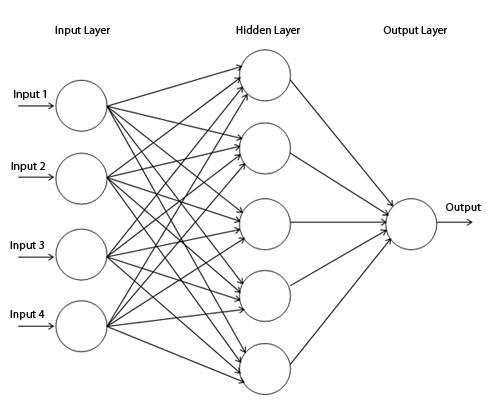
\includegraphics[width=0.45\textwidth]{network.jpg}
	\caption{A small feed-forward network with one hidden layer, and single output perceptron.
	Source: \href{http://www.codeproject.com/KB/dotnet/predictor/network.jpg}{Codeproject} 	}
	\label{fig:ff}
\end{figure}

\subsection{Basics of Learning}
After describing the model, the first question is:\\
\emph{what are the correct values for $\mathbf{w_P}$ for each $\mathbf{P}$ in network $N$?}

There are a lot of intuitive explanation how this problem should be approached and solved. For exhaustive investigation of the topic, see \cite{nnsdl}. 
Anyhow, in general this is still the most studied question in machine learning. 
Luckily if $N$'s performance can be measured, thanks to its feed-forward structure a \emph{numerical suggestion} can be defined as well, which tells how to change $\mathbf{w_P}$ to improve efficiency of $N$. In practice an $\mathbf{E}$ error function is defined, and the objective of the training is to reduce it. Without digging deep in math we can find an intuitive situation with the same results.\\

Take a perceptron $\mathbf{P}$ with input $\mathbf{x}$ of objects on a given picture of a cat. Suppose that this perceptron \emph{fires} (has high output value) when wheels are on the picture. It should remain silent when there are no round objects listed in 
$\mathbf{x}$, still it turns on, ruining the output of $N$, producing high $\mathbf{E}$.
Since we know the original label of the picture, we can tell which assumptions were wrong, and which were good - which to decrease, which to increase if the next time $N$ is given the same input. This information is distributed between the previous perceptrons which caused the actual to fail by simply multiplying the error with the weight corresponding to the previous node. Also with the information of how much the output of the actual node influenced the error, and with its input values, the significance of wrong $\mathbf{x_i}$s can be reduced, and important features' weights can be increased, which is actually finding a better $\mathbf{w_P}$.

The example concluded to the practical application of the so called \emph{Stochastic Gradient Descent}. Originally every samples in the training set should be introduced to the system before updating its weights and that would be the \emph{Gradient Descent}, but in  the hope that the samples falls in a subset of the whole space of all possible inputs, the algorithm uses mini-batches for the learning process. When the number of samples in the batches reduces to 1, the training is called on-line training. And if it happens on $N$ containing a single perceptron it is called \emph{Rosenblatt perceptron learning algorithm}.


\section{Inference}
Let us suppose that for a particular task an $\mathcal{F}$ is given, first what we have to understand is how input data 
$x \in \mathbb{X}$ (interchangeably $x_1$) is inferred.
First, assume that the data can be expressed as multi-dimensional matrix, like RGB pictures, audio recordings, gene maps.
Some networks preserve the spatial information i.e. feature extraction performed on images, 
while other instances operate on the whole input data i.e. processing audio samples in frequency domain.
Either way the output $y$ (or $y_L$) can be obtained by feeding $x$ to the network: 
$ y = \mathcal{F}(x)$
The core concept is that we can compose such an $\mathcal{F}$ function by applying multiple projections to $x$.
Practically that means sending input through the first layer, the second and all the way through to the last layer $L^{th}$, which output would be the value of $\mathcal{F}(x)$, the response of the network.
Therefore in terms of evaluating $\mathcal{F}(x)$ layer by layer, actually translates to a single function call, which can be unfolded to a sequence of embedded projections:
$$
    \mathcal{F}(x) = F_L \left( x_L \right) = F_L \left( y_{(L-1)} \right)
$$
$$
    F_L \left( y_{(L-1)} \right) = 
    F_L \left( F_{(L-1)} \left( x_{(L-1)} \right) \right) = F_L \left( F_{(L-1)}\left( \cdots F_1(x)\right)\right)
$$
Using the function composition operator $\circ$, rewritten in the classical notation:
\begin{equation}\label{eq:forward}
\begin{split}
    \mathcal{F}(x) = F_L \circ F_{(L-1)} \circ \cdots \circ F_1(x)
\end{split}
\end{equation}

The \ref{eq:forward} equation is the most fundamental idea behind feed-forward neural networks, namely the \emph{inference} or \emph{forward-propagation}
As mentioned above, every layer $l$ is represented by an $F_l$. 
The most basic layers are the \emph{Fully Connected} and \emph{Activation} layers.

\subsection{Fully Connected layer} 
These layers carry out the heavy-lifting of inference by performing linear projection and translation transformations. 
The operations are following the rules of basic linear algebra, where the input $x_{FC} \in \mathbb{R}^N$ and the output $y_{FC} \in \mathbb{R}^M$ are specified as real valued vectors.
The parameters of the layer $\phi_{FC}=(W, b)$ are the corresponding weights and biases of each perceptron node in the layer forming a \emph{weight matrix} $W \in \mathbb{R}^{M \times N}$ and a \emph{bias vector} $b \in \mathbb{R}^M$ respectively.
Therefore evaluating the output of the Fully Connected layer is the defined by the following:
\begin{equation}\label{eq:FC}
\begin{split}
    y_i = \left(\sum_i W_{i,j} \cdot x_j \right) + b_i \qquad &\in \mathbb{R}\\
    y = Wx + b \qquad &\in \mathbb{R}^M
\end{split}
\end{equation}
\subsection{Activation layer} 
Nodes in activation layers are introducing non-linearity to the network, by applying the same non-linear activation function to the corresponding output of the previous layer, performing element-wise operation.
These functions are essential for the network, since they increase the numerical stability: they \emph{squeeze} or \emph{mitigate} the input preventing the network from \emph{saturation} or \emph{explosion} (numerical of course). Conventionally the following functions are applied most often as activation function:
\begin{align*}
    \mathrm{Rectified Linear Unit (ReLU) := } &max(0, x) \\
    \mathrm{Hyperbolic Tangent (TanH) := }   &tanh(x) = \frac{2}{1+e^{-2x}}-1 \\
    \mathrm{SoftPlus (SP) := }   &ln(1+e^x) \\
    \mathrm{Sigmoid (S) := }  &\frac{1}{1+e^{-x}}
\end{align*}
The only constraint on these functions that they have to keep the dimension of the input, namely $F_{act}:\mathbb{R}^N \mapsto \mathbb{R}^N$.
\emph{Note:} These functions do not have any variable parameters, therefore activation layers cannot be trained.

\section{Measuring efficiency}
If the function $\mathcal{F}$ mentioned above is given, and satisfies our needs, then we are done.
However this is usually not the case, and finding the optimal $\mathcal{F}^*$ is the main challenge targeted by many branches of Machine Learning.
Despite it was proven, that standard multilayer
feed-forward networks are capable of approximating
any measurable function to any desired degree of
accuracy \cite{hornik1989multilayer}
if the goal function $\mathcal{F}^*$ is unknown, 
or too abstract to be \emph{measurable} (i.e. telling how funny a picture is), 
we cannot utilize the universal approximator.

\subsection{Loss} 
By reformulating the objective, we can define a Loss function $\mathcal{L}:\mathcal{F}(\mathbb{X}) \mapsto \mathbb{R}$,
which maps our candidate $\mathcal{F}$ network to a scalar field, that represents the general correctness of $\mathcal{F}$ over the space of possible inputs $\mathbb{X}$ -- the lower its value the better $\mathcal{F}$ is performing.
By doing so we may apply Machine Learning algorithms that would \emph{minimize} the Loss, therefore $\mathcal{F}$ would converge towards $\mathcal{F}^*$ implicitly.

\emph{Note:} In practical implementations $\mathcal{F}$ is not evaluated over the whole space of possible inputs, instead in the hope that a small subset of both \emph{training} and \emph{validating} samples called a mini-batch will approximate $\mathcal{L}(\mathcal{F})$ as well. Useful practices for reducing computing complexity and improving stability, and rate of convergence will be covered later.


\subsection{Supervised learning}
In cases where the parameters of $\mathcal{F}^*$ is not known but we know how it would map the input space $\mathbb{X} \mapsto \mathbb{Y}$, e.g. which character appears on the input image $x$, then we can define a set of previously \emph{labeled} pairs of input - solution sample which could be used later on for training, and evaluating performance of the network.

\subsection{Unsupervised learning}
When no labeled dataset is available, the network still can be used for extraction of hidden structure of the unlabeled samples. Later these instances are used as density estimators, or adapted as feature extractors for larger networks.
\textbf{Generative Networks.} Training such architectures can be done by feeding networks random noise as input and training them to reproduce given samples: $\mathcal{F}:\mathbb{R}^k \mapsto \mathbb{X}$, hence the name \emph{Generative Networks}.

\textbf{Auto-encoder Networks} The other frequently applied paradigm is setting the objective task to compress the input sample into a $h \in \mathbb{R}^k$ hidden representation vector that is able to preserve the key information about the original input, and either by symmetric (Restrictive Boltzmann Machines) or independent (Deep Belief networks) operations decompress the data.

In both cases hyper-parameter $k$ is intuitively the number of unlabeled features in the \emph{latent space} that the network will be able to categorize, i.e. correlation between different color intensities on pictures taken of stained brain samples.


\section{Adjusting parameters}
Generally speaking, applying Machine Learning algorithms boils down to the process of iteratively altering parameters $\phi$ of $\mathcal{F}$ to optimize the Loss.
Once $\mathcal{L}(\mathcal{F})$ is obtained, we can evaluate how changing the parameters would influence it -- evaluate the gradient $\nabla_\phi \mathcal{F}$ of the parameters  with regards to $\mathcal{L}$.

\subsection{Gradient Descent}
Updating $\phi$ by descending on the gradient slope with a small step size $\epsilon$ will decrease $\mathcal{L}$.
Enucleating the general form of Gradient Descent depends on the architecture of the network, but there is a main concept for doing so, called Backpropagation described by Werbos \emph{et al.} \cite{werbos1994roots}.

\paragraph{Train policies} 

\subsection{Backpropagation} 
Though networks can vary in shape and function, the representation of the succeeding layers, evaluated by embedded functions described in \ref{eq:forward} is a common feature. Each of these layers serve as nodes of the computational graph of the network. The type of the layer determines whether it can be updated or not: for \emph{Fully Connected} layers $\nabla_\phi F_{FC}$ is well defined, explained in the following example.

\paragraph{Toy example.} 
Assume $\mathcal{L}$ is given, and we have a fully connected network with 2 hidden layers, i.e. $L=3$, which maps a $N$ dimensional input vector $x$ to a $M$ dimensional output vector $y$, namely $\mathcal{F}:\mathbb{R}^N \mapsto \mathbb{R}^M$. The constraint on the parameters are:
\begin{itemize}
    \item[] $W^1$ of the first layer must have $N$ columns
    \item[] $W^3$ and the bias $b^3$ of the last layer must have $M$ rows, dimensions respectively.
    \item[] Number of rows of $W^l$ must match $dim(b^l)$ $3$ dimensional
    \item[] Number of columns of $W^l$ must match $dim(b^{(l-1)})$
\end{itemize} 
Then the evaluation unfolded would look like the following: 
$$y = \mathcal{F}(x) = F_3 \circ F_2 \circ F_1(x) = W^3(W^2(W^1(x)+b^1)+b^2)+b^3$$
For further usage and simplicity, I would like to fix these numbers.
Let $\mathcal{F}$ be a network with the following \emph{shape}: $\left[5, 4, 3\right] $
meaning that in each layer there are 5, 4, 3 neurons respectively, $M=3$ and all nodes are connected to the previous layer. The width of the input layer is not yet defined, let it be $N=10$. 
\emph{Note:} It is usually distracting and redundant to explicitly write the width of the outermost layers when testing different networks, because the input and the output layers must have fixed dimension for the same task, while the width of the hidden layers are varied.
Define an $L_2$ Loss function on the toy example. For one sample-label pair $(x,y^*)$ the $L_2$ Loss is:
\begin{equation}
    \mathcal{L}_2(\mathcal{F}) = \frac{1}{2} \sum_{i} (y_i^* - \mathcal{F}(x)_i)^2 = \frac{1}{2} \sum_{i} (y_i^* - y_i)^2
\end{equation}
$L_2$ is a universal Loss function, which is used in cases where the label space $\mathbb{Y}$ is continuous (e.g. floorspace, consumption and height of a house, based on the price: $\mathbb{R}^1 \mapsto \mathbb{R}^3$).

\section{Derivation} In the above evaluating of $\nabla_\phi \mathcal{F}$ can be done in two ways, namely by numerical approximation, or by analytical derivation, in the following I will discuss both.

\subsection{Numeric differentiation} Evaluating the numerical gradient (or difference) is an elementary, yet powerful operation, in which we would \emph{perturb}, or modify one parameter $\phi$ of our system $\mathcal{F}$ at once.
That is done by first adding $\phi^+$ and after subtracting $\phi^-$ a little amount $d\phi$ from the original $\phi$ and evaluate $\mathcal{L}^{\pm}=\mathcal{L}(\mathcal{F}_{\phi^{\pm}})$, namely the \emph{Loss} of the system in the modified state, yielding the numerical gradient in the following equation:

\begin{equation} \label{eq:numgrad}
    \frac{d\mathcal{L}(\mathcal{F})}{d\phi} = 
    \frac{\mathcal{L}^+ - \mathcal{L}^-}{2 d\phi} = 
    \frac{\mathcal{L}(\mathcal{F}_{\phi^+}) - \mathcal{L}(\mathcal{F}_{\phi^-})}{2 d\phi}
\end{equation}

\paragraph{Summary.} In a nutshell value of $\frac{d\mathcal{L}(\mathcal{F})}{d\phi}$ tells how changing the parameter $\phi$ by $d\phi$ would change the performance of the network. If it is positive then updating $\mathcal{F}$ by adding $d\phi$ to $\phi$ would result in higher Loss value, which is the opposite of our goal, so we just subtract it, if it is negative, than trivially we should add $d\phi$ to $\phi$ since it is making some good progress.

\subsection{Complexity} 
Though letting the computer do the hard work seems to be a good idea, it worths considering that the simple method above will be applied to every $\phi$ of $\mathcal{L}$.
It means that for the network in the toy example, we need to evaluate $\mathcal{L}(\mathcal{F})$ two times for each parameter in 
the weight matrices and the bias vectors of the network, totaling in 
$$\#(\phi) = 2\times\sum_{i=1}^3 N_{(i-1)}\cdot N_i + N_i = 2\times(10\cdot 5 + 5 ... + 4\cdot 3 + 3) = 188$$
Even if $\mathcal{F}$ is approximated by using $k$-sized mini-batches for evaluation it is still a computationally very expensive function, because the inference would result in the following number of operations of addition and multiplication:
$$\#(\mathrm{operations}) = k\times\sum_{i=1}^3 2\cdot N_{(i-1)}\cdot N_i + N_i = k \times 176$$
Therefore approximated with $k=10$ mini-batches would a single parameter update of a very tiny network would require total operations of:
\begin{equation}
    \#(\mathrm{total})=\#(\phi) \times k \times \#(\mathrm{operations}) = 188 \cdot 10 \cdot 176  = 330880
\end{equation}
Because both $\#(\phi)$ and $\#(\mathrm{operations})$ has complexity of $\mathcal{O}(N^2)$, one update will yield complexity of 
\begin{equation}
    \#(\mathrm{total})=\mathcal{O}(N^4)
\end{equation}
We can see that even for a shallow and relatively small network (industrial AI networks has billions of parameters, and uses much larger batches) described in the toy example the method is really costly.
That encourages us to derive our differentials on paper first, and use \emph{numerical gradient approximation} for checking our solution. Using \emph{Gradient Check} is essential when implementing new architectures, because it is a very efficient tool for debugging in comparison with updating. The method in a few words is about setting an error rate $\epsilon$, and decrease $d\phi$ until the numeric solution does not match the analytic solution with $1-\epsilon$ significance. If the analytic solution is incorrect the cycle will not terminate.

\subsection{Analytic differentiation}
Deriving the update by hand requires basic knowledge in calculus extended to multivariate cases, though since the operations are elementary, in general we must understand only three basic definitions to do so. 
Some formality before starting: we have three independent variables $x$, $y$, $z$ and functions $f$, $g$, $h$. The result of operations performed on variables, i.e. $x+2y$ can be represented by a function $f=x+2y$. 
If the value depends on a variable then it can be written explicitly, passing the variable as \emph{the argument} of the function $f(x,y)=x+2y$. 
For the sake of simplicity assume that the variables are not general objects from an abstract space, they are only real values: $x,y,z\in \mathbb{R}$. However the following description could be extended for the above-mentioned variables as well. For any one-dimensional function $f(x):\mathbb{R}\mapsto\mathbb{R}$ we say that the value represented by the function depends on the variable by the extent of its derivative. The derivative (or differential) of the function can be seen as an ideal case of \ref{eq:numgrad} where the perturbation would approach zero, namely:
\begin{equation}
    \frac{\partial f}{\partial x} = \lim_{dx\rightarrow 0}\frac{df(x)}{dx}= \lim_{dx\rightarrow 0} \frac{f(x+dx)-f(x-dx)}{2dx}
\end{equation}
\paragraph{Multiplication rule.}
Consider a value $x\cdot y \cdot z$ represented by $f(x,y,z)$. $f$ is now depending on three variables, we can define the measure of this dependency on one variable by the formal equation:
\begin{equation*}
\begin{split}
    \frac{\partial f}{\partial x} = \lim_{dx\rightarrow 0} \frac{f(x+dx,y,z)-f(x-dx,y,z)}{dx}
    &= \lim_{dx\rightarrow 0} \frac{((x+dx)\cdot y \cdot z)-((x-dx)\cdot y \cdot z)}{2dx} \\
    = \lim_{dx\rightarrow 0} \frac{(x+dx)-(x-dx)}{2dx} y z&= \lim_{dx\rightarrow 0} \frac{2dx}{2dx} yz= yz
\end{split}
\end{equation*}
We can apply the same method for each variable, the result will be the elements of the \emph{gradient} $\nabla f$
\begin{equation}\label{eq:multiplication}
    \frac{\partial f}{\partial x} = y z \qquad
    \frac{\partial f}{\partial y} = x z \qquad
    \frac{\partial f}{\partial z} = x y 
\end{equation} 
The important thing to understand that in a computational graph, a multiplicative node, which takes $N$ arbitrary parameters (or arguments), will have a \emph{partial derivative} for each variable its output is depending on. In general if these derivatives are represented as a vector, then it is called the gradient $\nabla f$ of $f$. Also the value of the derivative will be the product of all variables except the one of which we are computing the influence of on the output.

\paragraph{Addition rule.}
Consider a value $x\cdot y + x\cdot z$ represented by $g(x,y,z)$.
The change of $g$ with respect to $x$ is defined with the following shortened equation:
\begin{equation}\label{eq:addition}
    \frac{\partial g}{\partial x} = \lim_{dx\rightarrow 0} \frac{((x+dx)y +(x+dx)z)-((x-dx)y +(x-dx)z)}{dx}=y+z
\end{equation}
Notice that -- in the terms of computational graphs -- if a node contributes to other different operations (namely $x\cdot y$ and $x\cdot z$), 
than the derivative of each occurrence in \emph{later} values will be summed up. 

\paragraph{Chain rule.}
Let $f(x)=2x+3$ and $g(f)=5f$. Suppose that we would like to know the derivative of $g$ with respect to $x$.
At first we cannot do so, but there are two options: in the hope that substituting the value represented by $f$ into $g$ would not make the equation too complex we can unroll the references and rewrite $g(x)=5\cdot(2x + 3)$, or we could use the chain rule:
$$
    \frac{\partial g}{\partial x} = \lim_{dx \rightarrow 0} \frac{g(f(x+dx)) - g(f(x-dx))}{2dx}
$$

\begin{center}
    Assume that $f(x+dx)-f(x-dx) \neq 0$.
\end{center}

$$
    \lim_{dx \rightarrow 0} \frac{g(f(x+dx)) - g(f(x-dx) ) }{f(x+dx)-f(x-dx)} \cdot \frac{f(x+dx)-f(x-dx)}{2dx}
$$

\begin{equation}\label{eq:chain}
    \frac{\partial g}{\partial x} = \frac{\partial g}{\partial f} \cdot \frac{\partial f}{\partial x}
\end{equation}

Which is a formula of the products of partial derivative of $g$, that treats $f$ like a variable, and $f$ explicitly operating on variable $x$.
The derivative of $g$ with respect to variable $x$ is the product of the \emph{local derivative} of $g$ is $\frac{\partial g}{\partial f}=5$ and $\frac{\partial f}{\partial x}=2$ which equals $\frac{\partial g(x)}{\partial x}=\frac{\partial(5\cdot (2x + 3))}{\partial x} = 10$, the function strictly depending on $x$.
The important message is that we can interchangeably use function values and variables with a constraint that at a point, in an arbitrary depth there must be a real variable.
\emph{Note:} the statement above stands for computations with \emph{Acyclic Graph}, meaning that there should not be any feedbacks or loops -- no definitions like $f(g), g(f)$ or $f(f)$.
We will see that these rules play a very fundamental role in training networks.

\paragraph{vector notation}
Before drilling deep into mathematical equations, a small reminder: the following vector and matrix formulation is just a special annotation, 
using the rules above, which helps to make clear both the definition, and the computations done by the network when it is implemented. 
The vectors with partially derivatives inside are just representing \emph{real values}, arranged in a fancy way.
Every vector and matrix defined in forward propagation, has its corresponding derivative w.r.t. the Loss.
More trivially, if any value is depending on a list of variables $f(x_1, x_2 \cdots x_n) = f(\mathbf{x})$ (a vector) then there is a list of \emph{partial derivatives} w.r.t. to $f$ -- forming the gradient $\nabla f = \left(\frac{\partial f}{x_1}, \frac{\partial f}{x_1} \cdots \frac{\partial f}{x_N}\right)$. 
\emph{Notation}: When the vector notation is emphasized the variable name is conventionally written in bold font $\mathbf{x}$, or is underlined \underline{$x$}.
Because later the indexing would become too crowded, we only use the indexed notation when it is necessary, otherwise using $x$.

The next step is formulating the dependency of multiple functions on multiple variables.
As seen above, a multivariate function has its gradient vector --
in the same fashion as the list of variables were organized into vectors $\mathbf{x}$, values composed of them can also form a vector $F = (f_1, f_2 \cdots f_M)$, composing a multivalued function depending on the same variables.
Doing so yields a first-order derivative matrix, composed of gradient vectors $J=(\nabla f_1, \nabla f_2 \cdots \nabla f_M)^T$, called the \emph{Jacobian of $F$}.
The Jacobian has as many rows as output values $F$ has, and the same number of columns of the variables that $f_i$ is a function of.
$$
    J(F) = 
    \begin{pmatrix}
    \quad \nabla f_1 \quad \\ 
    \vdots \\ 
    \nabla f_M
    \end{pmatrix} 
    =
    \begin{pmatrix}
    \frac{\partial f_1}{\partial x_1} & \cdots & \frac{\partial f_1}{\partial x_N} \\ 
    \vdots & \ddots & \vdots \\ 
    \frac{\partial f_M}{\partial x_1} & \cdots & \frac{\partial f_M}{\partial x_N}
    \end{pmatrix} 
$$
The matrix and vector operations (such as addition and inner product) that can be performed on the derivative \emph{arrays} are identical defined in the inference section. That is important because product of derivatives introduced by the chain rule, can be applied as well for multidimensional array of derivatives too.

\paragraph{Fully Connected Layer}
Return to the toy example and begin with the last layer, with $3$ nodes. If a sample $x$ is inferred $\mathcal{F}(x)=y$, then the response of the network will be a vector of $dim(y) = 3$. If we took the $L_2$ \emph{distance} between the response and the goal $y^*$, then it would tell how far we are from the ideal, by a single scalar value. Since we want to minimize it, we have to adjust the parameters of the network, namely descend on the gradient slope. To get the small extent of the update we have to evaluate $\frac{\partial\mathcal{L}}{\partial \phi}$. 
Intuitively in the case we would like to correct the weights of a decision, it would require two things:
\begin{itemize}
    \item[] The original situation (the input of the $l^{th}$ layer $x_l$), which the decision was made in.
    \item[] The error on the decision -- the derivative $\delta^l$ of the Loss with regards to the decision.
\end{itemize}
Since $x_l$ is obtained via inference, what we have to calculate is $\delta^l$ for the $l^{th}$ layer in order to acquire the parameter gradient.
The first step is to evaluate the $\delta_L$, or the \emph{error} of the last layer's response $y^3$, namely $\delta^3 = \nabla_{y^3} \mathcal{L}$.
Begin with the first element: 
$$
    \delta_1^3 = 
    \frac{\partial \mathcal{L}}{\partial y_1} = 
    \frac{\partial}{\partial y_1}\frac{1}{2}\left((y^*_1 - y_1)^2 + (y^*_2 - y_2)^2 + (y^*_3 - y_3)^2\right) = y_1 - y^*_1
$$
\begin{center}
Expanding it to the whole array:
\end{center}
$$
    \delta^3 = \begin{pmatrix}
     \frac{\partial \mathcal{L}}{\partial y_1}\\ \\
    \frac{\partial \mathcal{L}}{\partial y_2} \\ \\
    \frac{\partial \mathcal{L}}{\partial y_3}
    \end{pmatrix} = \begin{pmatrix}
     \frac{\partial}{\partial y_1} \frac{1}{2}\sum_i(y_i^*-y_i)^2\\ \\
    \frac{\partial}{\partial y_2} \frac{1}{2}\sum_i(y_i^*-y_i)^2 \\ \\
    \frac{\partial}{\partial y^3_3}  \frac{1}{2}\sum_i(y_i^*-y_i)^2
    \end{pmatrix} = \begin{pmatrix}
     {y_1-y^*_1}\\ \\
     {y_2-y^*_2}\\ \\
     {y_3-y^*_3}
    \end{pmatrix} 
$$
Consider the following notation:
$
    \delta^3_i = (y^*_i - y_i)
$, 
called parametric vector notation. Writing arrays in this way, saves a lot of space. However, when this notation gets jammed with indexes, it is useful to write down explicitly the whole array for clarification.

Now we have exact values of $\delta^3$ and $x^3$, so we can calculate how should the weights in $W^3$ be changed in order to get a better network.
Taking the first perceptron of the layer, it has a weight $W^3_1=(w_{1,1}, w_{1,2}, w_{1,3}, w_{1,4})$ for each output of the previous layer.
Suppose that this neuron had to tell how rounded is the object on an image sample, 
and the $i^{th}$ neuron of the $2^{nd}$ layer fires when it recognizes sharp edges.
Of course it would be bad if our neuron had a large weight on $x^3_i$. 
If this node performs poorly because of $x^3_i$, then it would contribute a lot to the Loss function while inferring sharp objects, with its output $y_1$ being far away from $y^*_1$, resulting in a positive $\delta^3_1$. 
In case of $x^3_i = 0$, the weight $w_{1,i}$ has nothing to do with the error $\delta^3_1$ of the neuron.
Notice that the error of each weight (w.r.t $\mathcal{L}$) should be proportional to the error and the input as well: $\frac{\partial \mathcal{L}}{\partial w_{1,i}}=x^3_i \cdot \delta^3_1$.
Now assume that a picture of an origami sculpture was inferred and the $i^{th}$ node of the second layer worked correctly. Both $x^3_i$ and $\delta^3_1$ is positive but the weight should be decreased: that is why we will take the negative of the derivative for updating $w_{1,i}$.
Substituting $i=1,2,3,4$ into $\frac{\partial \mathcal{L}}{\partial w_{1,i}}$ yields a gradient of $\mathcal{L}$ with regards to the weights of the first neuron of the last layer. Doing so for each neurons in the layer would result in 3 gradient vectors $\nabla_{W_1} \mathcal{L}$, $\nabla_{W_2} \mathcal{L}$ and $\nabla_{W_3 }\mathcal{L}$ which is practically stacked to make a matrix which can be later added element-wisely to the weight matrix $W$.
\begin{equation}
\nabla_W \mathcal{L} = 
\left(\frac{\partial \mathcal{L}}{\partial W_{i,j}}\right) \Longrightarrow 
\begin{pmatrix}
\frac{\partial \mathcal{L}}{\partial W_{1,1}} & \frac{\partial \mathcal{L}}{\partial W_{1,2}} & \frac{\partial \mathcal{L}}{\partial W_{1,3}} & \frac{\partial \mathcal{L}}{\partial W_{1,4}} \\ \\
\frac{\partial \mathcal{L}}{\partial W_{2,1}} & \frac{\partial \mathcal{L}}{\partial W_{2,2}} & \frac{\partial \mathcal{L}}{\partial W_{2,3}} & \frac{\partial \mathcal{L}}{\partial W_{2,4}} \\ \\
\frac{\partial \mathcal{L}}{\partial W_{3,1}} & \frac{\partial \mathcal{L}}{\partial W_{3,2}} & \frac{\partial \mathcal{L}}{\partial W_{3,3}} & \frac{\partial \mathcal{L}}{\partial W_{3,4}}
\end{pmatrix} = 
\begin{pmatrix}
 x_1 \delta_1 &  x_2 \delta_1 &  x_3 \delta_1 &  x_4 \delta_1 \\ \\
 x_1 \delta_2 &  x_2 \delta_2 &  x_3 \delta_2 &  x_4 \delta_2 \\ \\
 x_1 \delta_3 &  x_2 \delta_3 &  x_3 \delta_3 &  x_4 \delta_3
\end{pmatrix}
\end{equation}



\paragraph{Activation Layer.} To have a better grasp on how to extend the rules (\ref{eq:multiplication}, \ref{eq:addition}, \ref{eq:chain}) for neural networks in practice, consider a 